% Options for packages loaded elsewhere
\PassOptionsToPackage{unicode}{hyperref}
\PassOptionsToPackage{hyphens}{url}
%
\documentclass[
  11pt,
]{article}
\usepackage{lmodern}
\usepackage{amssymb,amsmath}
\usepackage{ifxetex,ifluatex}
\ifnum 0\ifxetex 1\fi\ifluatex 1\fi=0 % if pdftex
  \usepackage[T1]{fontenc}
  \usepackage[utf8]{inputenc}
  \usepackage{textcomp} % provide euro and other symbols
\else % if luatex or xetex
  \usepackage{unicode-math}
  \defaultfontfeatures{Scale=MatchLowercase}
  \defaultfontfeatures[\rmfamily]{Ligatures=TeX,Scale=1}
\fi
% Use upquote if available, for straight quotes in verbatim environments
\IfFileExists{upquote.sty}{\usepackage{upquote}}{}
\IfFileExists{microtype.sty}{% use microtype if available
  \usepackage[]{microtype}
  \UseMicrotypeSet[protrusion]{basicmath} % disable protrusion for tt fonts
}{}
\makeatletter
\@ifundefined{KOMAClassName}{% if non-KOMA class
  \IfFileExists{parskip.sty}{%
    \usepackage{parskip}
  }{% else
    \setlength{\parindent}{0pt}
    \setlength{\parskip}{6pt plus 2pt minus 1pt}}
}{% if KOMA class
  \KOMAoptions{parskip=half}}
\makeatother
\usepackage{xcolor}
\IfFileExists{xurl.sty}{\usepackage{xurl}}{} % add URL line breaks if available
\IfFileExists{bookmark.sty}{\usepackage{bookmark}}{\usepackage{hyperref}}
\hypersetup{
  pdftitle={New and old ways to chase a rabbit: Differential item functioning detection methods},
  hidelinks,
  pdfcreator={LaTeX via pandoc}}
\urlstyle{same} % disable monospaced font for URLs
\usepackage[margin=1in]{geometry}
\usepackage{longtable,booktabs}
% Correct order of tables after \paragraph or \subparagraph
\usepackage{etoolbox}
\makeatletter
\patchcmd\longtable{\par}{\if@noskipsec\mbox{}\fi\par}{}{}
\makeatother
% Allow footnotes in longtable head/foot
\IfFileExists{footnotehyper.sty}{\usepackage{footnotehyper}}{\usepackage{footnote}}
\makesavenoteenv{longtable}
\usepackage{graphicx,grffile}
\makeatletter
\def\maxwidth{\ifdim\Gin@nat@width>\linewidth\linewidth\else\Gin@nat@width\fi}
\def\maxheight{\ifdim\Gin@nat@height>\textheight\textheight\else\Gin@nat@height\fi}
\makeatother
% Scale images if necessary, so that they will not overflow the page
% margins by default, and it is still possible to overwrite the defaults
% using explicit options in \includegraphics[width, height, ...]{}
\setkeys{Gin}{width=\maxwidth,height=\maxheight,keepaspectratio}
% Set default figure placement to htbp
\makeatletter
\def\fps@figure{htbp}
\makeatother
\setlength{\emergencystretch}{3em} % prevent overfull lines
\providecommand{\tightlist}{%
  \setlength{\itemsep}{0pt}\setlength{\parskip}{0pt}}
\setcounter{secnumdepth}{5}
\usepackage{amsmath}
\DeclareMathOperator*{\argmax}{arg\,max}
\DeclareMathOperator*{\argmin}{arg\,min}
\usepackage{float}
\usepackage[autostyle, english = american]{csquotes}
\setlength{\parindent}{4em}
\setlength{\parskip}{2em}
\usepackage{setspace}\doublespacing
\AtBeginEnvironment{tabular}{\singlespacing}
\usepackage{natbib}
\usepackage{booktabs}
\usepackage{longtable}
\usepackage{array}
\usepackage{multirow}
\usepackage{wrapfig}
\usepackage{float}
\usepackage{colortbl}
\usepackage{pdflscape}
\usepackage{tabu}
\usepackage{threeparttable}
\usepackage{threeparttablex}
\usepackage[normalem]{ulem}
\usepackage{makecell}
\usepackage{xcolor}

\title{New and old ways to chase a rabbit:\\
Differential item functioning detection methods}
\usepackage{etoolbox}
\makeatletter
\providecommand{\subtitle}[1]{% add subtitle to \maketitle
  \apptocmd{\@title}{\par {\large #1 \par}}{}{}
}
\makeatother
\subtitle{Ben Stenhaug\\
Stanford University}
\author{}
\date{\vspace{-2.5em}}

\begin{document}
\maketitle
\begin{abstract}
summarize propose extensions insist as dif as student property and on communicating uncertainty
\end{abstract}

{
\setcounter{tocdepth}{5}
\tableofcontents
}
\clearpage

\hypertarget{to-do}{%
\section{TO DO}\label{to-do}}

\begin{itemize}
\tightlist
\item
  be sure all my directions match. i think i switched everything to be item easiness at some point but not sure if i did it throughout
\end{itemize}

\hypertarget{introduction}{%
\section{Introduction}\label{introduction}}

Inspired by Camilli (\protect\hyperlink{ref-camilli1992conceptual}{1992}), we think differential item functioning (DIF) as bias against a group of students that manifests when an item response model with too few ability dimensions is imposed. From this perspective, the term \enquote{differential item functioning} is, perhaps, a misnomer as DIF is a property of the student, not the item. For example, Ackerman (\protect\hyperlink{ref-ackerman1992didactic}{1992}) describes a scenario in which a test intends to measure a student's math ability, but performance also depends on their verbal ability. In this case, math ability is the \enquote{target ability,} and verbal ability is the \enquote{nuisance ability.} Fitting a unidimensional item response model to this test results in students with low verbal ability receiving a score systematically lower than their true math ability; therein lies DIF.

Contrarily, the usual setup of DIF simulation studies frames DIF as a property of the item. For example, Kopf, Zeileis, and Strobl (\protect\hyperlink{ref-kopf2015framework}{2015}) simulate students as belonging to either a reference or focal group. They fix the item easinesses for the reference group, \({b_j}^{\text{ref}}\), to values from a previous study. They set item easinesses for the focal group to \({b_j}^{\text{foc}} = {b_j}^{\text{ref}}\) for items without DIF and \({b_j}^{\text{foc}} = {b_j}^{\text{ref}} + 0.6\) for items with DIF, where 0.6 is the magnitude of DIF in logits. They simulate student ability \({\theta_i}^{\text{ref}} \sim N(0,1)\) for students in the reference group and \({\theta_i}^{\text{foc}} \sim N(-1,1)\) for students in the focal group. They generate item responses according to the Rasch model, which specifies that the probability of student \(i\) responding correctly to item \(j\) is \[P(y_{ij} = 1 | \theta_i, b_j) = \sigma(\theta_i + b_j)\] where \(\sigma(x) = \frac{e^x}{e^x + 1}\) is the standard logistic function.

We find it informative to describe simulation conditions in terms of multidimensional abilities as opposed to item parameters that vary across groups. For example, to translate the Kopf, Zeileis, and Strobl (\protect\hyperlink{ref-kopf2015framework}{2015}) simulation from the DIF-as-item-property view to the DIF-as-student-property view, item easiness is set to what was previously \({b_j}^{\text{ref}}\) for all students. Student ability is expanded to two dimensions, the target ability dimension and nuisance ability dimension. The target ability is what was previously just ability where \({\theta_i}^{\text{ref}} \sim N(0,1)\) for students in the reference group and \({\theta_i}^{\text{foc}} \sim N(-1,1)\) for students in the focal group. The nuisance ability is set to \({\eta_i}^{\text{ref}} = 0\) for the reference group and \({\eta_i}^{\text{ref}} = -1\) for the focal group. We now need to use a 2PL model where the slope on target ability \(a_{1j} = 1\) for all items (consistent with the Rasch model) and the slope on nuisance ability \(a_{2j} = 0.6\) for all items with DIF, and \(a_{2j} = 0\) otherwise. Again, 0.6 is the magnitude of DIF in logits. According to the two-dimensional 2PL model, the probability student \(i\) responding correctly to item \(j\) is
\begin{align}
    P(y_{ij} = 1 | \theta_i, \eta_i, a_{1j}, a_{2j}, b_j) = \sigma(a_{1j}\theta_i + a_{2j}\eta_i + b_j).
\end{align}
This translation between views makes explicit that nearly all DIF simulation studies have, perhaps suboptimally, examined the unrealistic scenario in which there is no variation in nuisance ability for students in the same group.

If we insist on describing simulation conditions from the DIF-as-student-property view, one might wonder the following: Why not fit a multidimensional item response model which describes the data fully instead of looking for bias in a lower dimensional model? Camilli (\protect\hyperlink{ref-camilli1992conceptual}{1992}) tested this idea with the goal of a \enquote{more satisfying description of the secondary abilities} {[}p.~144{]}. He found that the rotational indeterminacy of item response models is challenging to overcome and concluded that \enquote{a priori knowledge of the true factor structure} is necessary {[}p.~144{]}. It's hard to imagine how one would have such knowledge. Therefore, the best approach, which the DIF literature has nearly unanimously taken, is to fit unidimensional item response models and then look for bias manifesting in the item parameters.

\hypertarget{dif-methods}{%
\section{DIF methods}\label{dif-methods}}

Psychometricians have long been in search of the perfect DIF detection method. In this section, we summarize existing DIF methods and propose extensions of those methods. We limit our discussion to IRT-based methods. As a result, we avoid methods like the Mantel-Haenszel procedure (Holland and Thayer \protect\hyperlink{ref-holland1986differential}{1986}), which muddies the waters by moving away from the IRT framework, and has been shown to perform no better --- and in some cases worse --- than IRT-based methods (Swaminathan and Rogers \protect\hyperlink{ref-swaminathan1990detecting}{1990}). For simplicity, we focus on the Rasch model to isolate the fundamental issues in DIF detection. And, in search of a coherent framework, we sometimes edit names of existing methods. We recognize that others have done the same (e.g.~Kopf, Zeileis, and Strobl \protect\hyperlink{ref-kopf2015framework}{2015}) and that we risk contributing to the proliferation of names.

We use a simple, one-run simulation to demonstrate the methods: 10,000 reference group students and 10,000 focal group students taking an eight-item test. Target ability is simulated \({\theta_i}^{\text{ref}} \sim N(0,1)\) for students in the reference group and \({\theta_i}^{\text{foc}} \sim N(-1,1)\) for students in the focal group. Nuisance ability is set to \({\eta_i}^{\text{ref}} = 0\) and \({\eta_i}^{\text{ref}} = -1\). The slope on target ability is set to \(a_{1j} = 1\) for all items, and the slope on nuisance ability is set to \(a_{2j} = 0.5\) for the last three items (the items with DIF) and \(a_{2j} = 0\) otherwise. From the DIF-as-item-property view, there is no nuisance ability. Instead, \({b_j}^{\text{foc}} = {b_j}^{\text{ref}}\) for the first five items and \({b_j}^{\text{foc}} = {b_j}^{\text{ref}} - 0.5\) for the last three items.

In general, we denote the mean ability of the reference and focal group as \(\mu^\text{ref}\) and \(\mu^\text{foc}\), respectively. We follow the common and inconsequential practice of identifying the scale by setting \(\mu^\text{ref} = 0\). The fundamental challenge for a DIF method is to first get an estimate for \(\mu^\text{foc}\), \(\hat\mu^\text{foc}\). How can group ability be disentangled from the possibility that items are biased? The most common approach is to identify a group of anchor items that are assumed to be DIF-free. These items are used to get \(\hat\mu^\text{foc}\).

\hypertarget{anchor-items}{%
\subsection{Anchor items}\label{anchor-items}}

\hypertarget{all-others-as-anchors}{%
\subsubsection{All-others-as-anchors}\label{all-others-as-anchors}}

Meade and Wright (\protect\hyperlink{ref-meade2012solving}{2012}) compared the most commonly used methods and unequivocally recommended the all-others-as-anchors (AOAA). AOAA tests each item for DIF one at a time using all of the other items as anchors. For example, when testing the first item for DIF, all of the other items are used as anchors. This is done using a likelihood ratio test that compares the baseline model, where all item parameters are fixed across groups, to the flexible model, where the parameters of the tested item are freed across groups (Thissen, Steinberg, and Wainer \protect\hyperlink{ref-thissen1993detection}{1993}). Then, when testing the second item for DIF, once again all of the other items (including the first item) are used as anchors, and so on. The items for which the flexible model outperforms the baseline model (typically based on a chi-squared test) are identified as having DIF and the rest of the items become anchor items.

Edelen et al. (\protect\hyperlink{ref-edelen2006identification}{2006}) used AOAA to look for DIF between the English and Spanish versions of the 21-item Mini-Mental State Examination and found that 10 of the 21 items exhibited DIF. How can we be sure its those 10 items and not the other 11 items with DIF? We can't be. Implicit in the use of AOAA is the assumption that all items not being tested do not exhibit DIF, which is, of course, impossible. More practically, it is thought that AOAA will perform well if a small minority of items have DIF or the DIF is balanced such that some items are biased against the focal group and others are biased against the reference group. Undesirably, most applications of DIF methods and many simulation studies do not make explicit the assumptions of the DIF method (Strobl et al. \protect\hyperlink{ref-strobl2018anchor}{2018}). In this way, psychometricians might benefit from adopting economists' habit of explicitly stating assumptions and debating their plausibility.

Researchers have noticed the circular logic of AOAA, but have mostly described it indirectly by pointing out inflated Type I errors in simulation studies (Stark, Chernyshenko, and Drasgow \protect\hyperlink{ref-stark2006detecting}{2006}). A simple thought experiment illustrates how AOAA fails: Imagine a test with a sufficiently large number of students and three items where the first item has DIF, and the other two do not. Using AOAA, all items test positive for DIF. The last two items incorrectly test positive because including the first item in the anchor set causes the group ability difference to be misestimated. This phenomenon of items with real DIF inducing the appearance of DIF in other items was only indirectly discussed in the literature until Andrich and Hagquist (\protect\hyperlink{ref-andrich2012real}{2012}) coined the term \enquote{artificial DIF.}

\hypertarget{all-others-as-anchors-all-significant}{%
\paragraph{All-others-as-anchors-all-significant}\label{all-others-as-anchors-all-significant}}

One way to attempt to counter artificial DIF is with purification through iterative anchor selection. For example, Drasgow (\protect\hyperlink{ref-drasgow1987study}{1987}) started with AOAA, removed items displaying DIF from the anchor set, then repeated the process iteratively --- with items that have been removed from the anchor set allowed to have free parameters across groups in both the baseline and flexible model --- until no more items tested positively. Kopf, Zeileis, and Strobl (\protect\hyperlink{ref-kopf2015framework}{2015}) named this technique Iterative-backward-AOAA with \enquote{backward} (as in reverse, not incorrect) referring to beginning with the assumption that all items are DIF-free. We find it clearer to refer to this method as all-others-as-anchors-all-significiant (AOAA-AS). Appending all-significant indicates that anchor selection is done iteratively with all items that show statistical significance for DIF being removed from the anchor set.

AOAA-AS might seem like an improvement but it doesn't solve a fundamental problem of AOAA: What do we do when all items test positive for DIF? With a sufficient sample size and at least one item with DIF, this will necessarily be the case. In our thought experiment, we get the same result with AOAA-AS as we did with AOAA: All items test positive for DIF and there are no anchor items. Kopf, Zeileis, and Strobl (\protect\hyperlink{ref-kopf2015framework}{2015}) encountered precisely this problem in their simulation study and chose to select a single anchor item randomly. Woods (\protect\hyperlink{ref-woods2009empirical}{2009}) suggested a more straightforward, one-step method which uses AOAA and selects the, say, four items that exhibit the least amount of DIF. It's unclear if one should proceed if those four items display DIF themselves.

\hypertarget{all-other-as-anchors-one-at-a-time}{%
\paragraph{All-other-as-anchors-one-at-a-time}\label{all-other-as-anchors-one-at-a-time}}

We propose an extension of these methods, all-others-as-anchors-one-at-a-time (AOAA-OAT), which, to our knowledge (and surprise), has not previously been proposed. Like AOAA-AS, AOAA-OAT starts with AOAA, but only the single item exhibiting the most DIF, based on the \(\chi^2\) test statistic, is removed from the anchor set. The process continues iteratively until no new items display DIF. AOAA-OAT and AOAA-AS are similar in that they are both iterative; the difference is that AOAA-OAT takes the more conservative approach of removing only one item in each iteration as opposed to all items that test positive for DIF. As a result, AOAA-OAT is less likely to arrive at the wrong conclusion because of artifical DIF.

Applying AOAA-OAT to our thought experiment demonstrates its effectiveness. The initial AOAA removes the real DIF item from the anchor set because it exhibits the most DIF. In the next step, both of the other items test negative for DIF, and we arrive at the correct conclusion. AOAA-OAT has two assumptions: First, that at least one item does not have DIF, and second, that the majority of items do not have DIF.

\hypertarget{summary-and-performance}{%
\paragraph{Summary and performance}\label{summary-and-performance}}

Table \ref{table:themethods} summarizes the three all-others-as-anchors methods. It's useful to remember that AOAA is not an iterative procedure, while the methods with a hyphen, AOAA-OAT and AAOA-AS, are iterative procedures with AOAA-OAT being our new, more conservative method.

\begin{table}[H]
\caption{EDIT THIS}
\centering
\begin{tabular}{|p{2.5cm}|p{6cm}|p{4cm}|}
\toprule

Method & Description & Literature \\

\midrule

AOAA & Test if each item has DIF by using all of the other items as anchors (not iterative). & Originally proposed by \cite{lord1980} and formalized by \cite{thissen1993detection} \\\hline

AOAA-AS & The first iteration is AOAA. All items that test positive for DIF are removed from the anchor set. Continue iterating until no new items test positive for DIF. & Proposed by \cite{drasgow1987study} \\\hline

AOAA-OAT & The first iteration is AOAA. Only the item that shows the most extreme DIF is removed from the anchor set. Continue iterating until no new items test positive for DIF. & To our knowledge, not proposed or used previously \\

\bottomrule
\end{tabular}
\label{table:themethods}
\end{table}

{[}ADD IN SIMULATION RESULTS{]}

\hypertarget{clustering-items}{%
\subsubsection{Clustering items}\label{clustering-items}}

Bechger and Maris (\protect\hyperlink{ref-bechger2015statistical}{2015}) proposed choosing anchor items by identifying clusters of items that function similarly and then choosing one of those clusters to be the \enquote{anchor cluster.} They pointed out that one way around the unidentifiability issue is to consider relative item parameters. For each group, the relative easinesses for each pair of items can be stored in the matrix \(\mathbf{R}^{\text{ref}}\) with entries \({R_{xy}}^{\text{ref}} = {b_x}^{\text{ref}} - {b_y}^{\text{ref}}\). The ultimate matrix of interest is \(\Delta \mathbf{R} \equiv \mathbf{R}^{\text{ref}}-\mathbf{R}^{\text{foc}}\) which is the \enquote{differences between groups in the pairwise differences in (easiness) between items} {[}p.~323{]}.

The general idea of identifying clusters of items is intriguing. However, their approach is needlessly complicated and they did not describe a process for moving from \(\Delta \mathbf{R}\) to a set of anchor items. Pohl, Stets, and Carstensen (\protect\hyperlink{ref-pohl2017cluster}{2017}) extended their work by proposing one such process. \(\Delta \mathbf{R}\) is skew-symmetric and of rank 1, which means that all information is contained in a single row or column. Accordingly, they use k-means clustering on just the first column of \(\Delta \mathbf{R}\) where the number of clusters, k, is chosen by minimizing BIC. They suggest using a combination of cluster size, cluster homogeneity, and cluster parameter precision to choose which of the clusters is the anchor cluster. Unfortunately, in their simulation study, they find that BIC identifies only a single cluster, so they end up using all of the items as anchors.

We propose a new cluster-based approach, which we call \enquote{equal means clustering} (EMC). Instead of working with an arbitrary column from \(\Delta \mathbf{R}\), we work with the vector \(\tilde{\mathbf{d}}\) of differences in item easiness, \(\tilde{d_j} = \tilde{b_j}^\text{ref} - \tilde{b_j}^\text{foc}\), where the model is identified by setting \(\mu^\text{foc} = 0\) (recall \(\mu^\text{ref}\) is always set to \(0\), thus the name \enquote{equal means clustering}). This results in all differences in performance --- either from group ability differences or DIF --- manifesting in the item easiness difference parameter \(\tilde{d_j}\). The tilde is used to denote parameters estimated with \(\mu^\text{foc}\) arbitrarily set to \(0\).

Instead of choosing k with BIC, we use the gap statistic method recommended by Hastie, Tibshirani, and Walther (\protect\hyperlink{ref-hastie2001estimating}{2001}). The largest cluster is chosen as the anchor cluster. If there is a tie for the largest cluster, the cluster with the lowest standard deviation of \(\tilde{\mathbf{d}}\) is selected. This process makes the assumption that the largest cluster (but necessarily the majority) of items do not contain DIF.

OUR SIMULATION RESULTS

\begin{tabular}{l|r|r|r|r|l}
\hline
item & a\_ref\_easy & b\_foc\_easy & difference\_in\_easy & cluster & anchor\\
\hline
item1 & -0.5638213 & -1.5520228 & 0.9882015 & 1 & TRUE\\
\hline
item2 & -0.2618317 & -1.2619495 & 1.0001178 & 1 & TRUE\\
\hline
item3 & 1.5747215 & 0.5456186 & 1.0291029 & 1 & TRUE\\
\hline
item4 & 0.0521493 & -0.9183001 & 0.9704494 & 1 & TRUE\\
\hline
item5 & 0.1335217 & -0.8599758 & 0.9934975 & 1 & TRUE\\
\hline
item6 & 1.6971526 & 0.1926118 & 1.5045408 & 2 & FALSE\\
\hline
item7 & 0.4629179 & -1.0572527 & 1.5201706 & 2 & FALSE\\
\hline
item8 & -1.2953061 & -2.8759098 & 1.5806036 & 2 & FALSE\\
\hline
\end{tabular}

\hypertarget{analyst-chooses}{%
\subsubsection{Analyst chooses}\label{analyst-chooses}}

DIF methods are generally designed to automatically detect DIF without any human judgement. On the other hand, it can be useful to present information to the analyst in a way that empowers them to see DIF and potentially even select the anchor items.

We propose a technique, the \enquote{equal means, multiple imputation logit graph} (EM-MILG), which presents information about potential DIF to the analyst. Like EMC, EM-MILG begins by fitting a unidimensional Rasch model to the data that is identified by setting \(\mu^\text{foc}\) to \(0\). Again, the result is that all differences in performance manifest in \(\tilde{\mathbf{d}}\). To get a sense of variation in each \(\tilde{{d_j}}\), the item parameter covariance matrix is estimated using Oakes' identity (Chalmers \protect\hyperlink{ref-chalmers2018numerical}{2018}). Then, multiple imputations (MI) (Yang, Hansen, and Cai \protect\hyperlink{ref-yang2012characterizing}{2012}) are used to estimate the distribution of \(\tilde{d_j}\) for every item. These are the distributions displayed in the EM-MILG. The method is inspired in part by Pohl, Stets, and Carstensen (\protect\hyperlink{ref-pohl2017cluster}{2017}) who fit a model with both the reference and focal group means set to 0 in a pedagogical example, and Talbot III (\protect\hyperlink{ref-talbot2013taking}{2013}) who fixed both pre-test and post-test means to 0 in order to estimate item-specific learning gains.

Figure \ref{fig:emmilg} shows the EM-MILG for our simulated data. It cannot be stated strongly enough that the EM-MILG contains all possible information about the difference in group performance. The challenge, then, is to select the anchor items. The analyst might assume that --- because there are five items where the reference group outperforms the focal group by 1 logit and only three items where the difference is 1.5 logits --- items 1-5 are unbiased and can be used as anchor items.

\begin{figure}[H]

{\centering 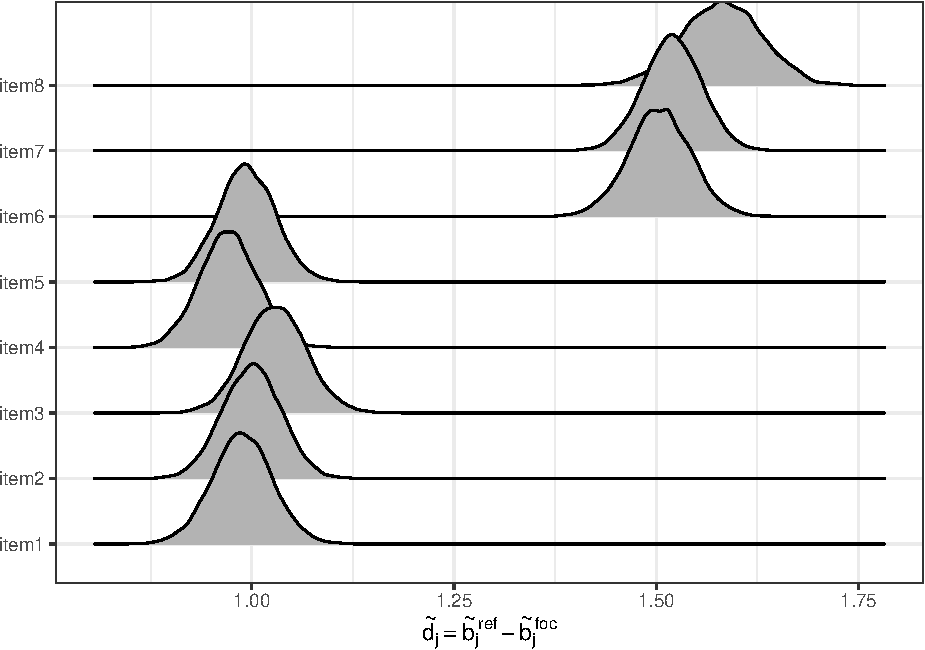
\includegraphics[width=0.7\linewidth]{paper_files/figure-latex/emmilg-1} 

}

\caption{The equal means multiple imputations logit graph (EM-MILG) shows the distribution of how many logits the reference group outperforms the focal group by on each item.}\label{fig:emmilg}
\end{figure}

After choosing the anchor items, the model is refit. The new model is identified by setting \(d_j = 0\) for the anchor items, instead of by setting \(\mu^\text{foc}\) to \(0\). The same process of using multiple imputations to estimate the distribution of \(d_j\) can be used with the new model. Because the equal means assumption is not made, we refer to the resulting graph as a multiple imputations logit graph (MILG). In our simulation, selecting the first five items as anchors correctly results in \(\hat d_j \approx 0.5\) for the items with DIF as is shown in the MILG in Figure \ref{fig:milg}.

\begin{figure}[H]

{\centering 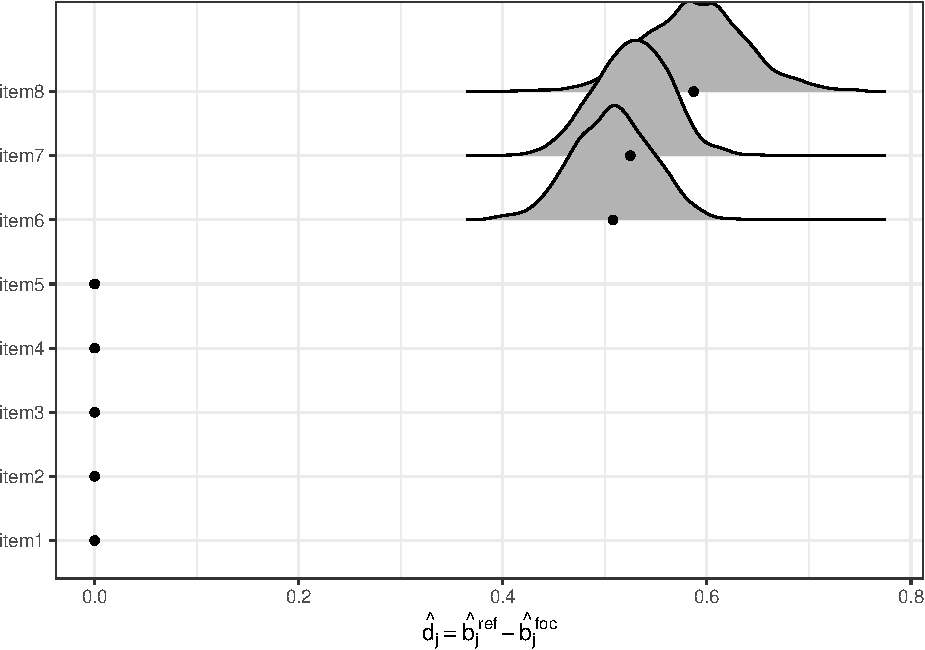
\includegraphics[width=0.7\linewidth]{paper_files/figure-latex/milg-1} 

}

\caption{The multiple imputations logit graph (MILG) shows the distribution of DIF against the focal group. Anchor items are fixed to 0.}\label{fig:milg}
\end{figure}

One of our key concerns with typical DIF methods is that they can lull the analyst into a false sense of security. Too often, the analyst chooses a method, implements it, and then proceeds as if the method certainly identified the correct anchor items. The EM-MILG combats this concern by presenting all information clearly to the analyst. In the previous example, the analyst may be weary of their results having seen how arbitrary it was to conclude that the first five and not the last three items are unbiased. Even when other DIF methods are used, the analyst can use the EM-MILG as a first step in order to give them a sense of their item response data. And, of course, the MILG can be used to visualize DIF anytime a model is fit using anchor items, not just when the first step involves the EM-MILG.

\hypertarget{anchor-points}{%
\subsection{Anchor points}\label{anchor-points}}

The previously discussed DIF methods select a set of anchor items, whether that selection is done by an algorithm or the analyst. The anchor items are used to estimate \(\hat \mu^\text{foc}\). An alternative strategy is to directly select the anchor point, \(\mu^{\star\text{foc}}\). Anchor point methods have the advantage of not requiring the assumption that any particular item is DIF-free, and, therefore, all items can be tested for DIF. The question then becomes the following: How do we select the anchor point?

\hypertarget{gini-index}{%
\subsubsection{Gini index}\label{gini-index}}

Strobl et al. (\protect\hyperlink{ref-strobl2018anchor}{2018}) suggest using the Gini index (\protect\hyperlink{ref-gini1912variabilita}{1912}) to select the anchor point. The Gini index is typically used to measure the inequality of wealth distribution in a country. For example, South Africa typically has the highest Gini index of all measured countries, meaning that it is the country with the most unequal wealth distribution Chitiga, Sekyere, and Tsoanamatsie (\protect\hyperlink{ref-chitiga2015income}{2015}). In general, the Gini index \enquote{takes high values if, for example, a small minority of persons has a lot of wealth while the vast majority has very little} (Strobl et al. \protect\hyperlink{ref-strobl2018anchor}{2018}, 7).

The anchor point, \(\mu^{\star\text{foc}}\), is selected by maximizing the Gini index. The intuition and assumption is that some items might have bias but the majority do not. Denoting a function that calculates the Gini index from a vector of non-negative elements as \(G(\mathbf{x})\),
\[
\mu^{\star\text{foc}} = \mathop\mathrm{arg\,max}_{\mu^\text{foc}} G(|\mu^\text{foc} + \tilde{\mathbf{d}}|)
\]
where \(\mu^\text{foc} \in (-\infty, \infty)\) and \(\mu^\text{foc}\) is added to each element of \(\mathbf{d}\).

For the simulated data, Figure \ref{fig:ginipath} shows the gini coefficient at a variety of possible values for \(\mu^\text{foc}\). The anchor point is \(\mu^\text{foc} = -0.99\).

\begin{figure}[H]

{\centering 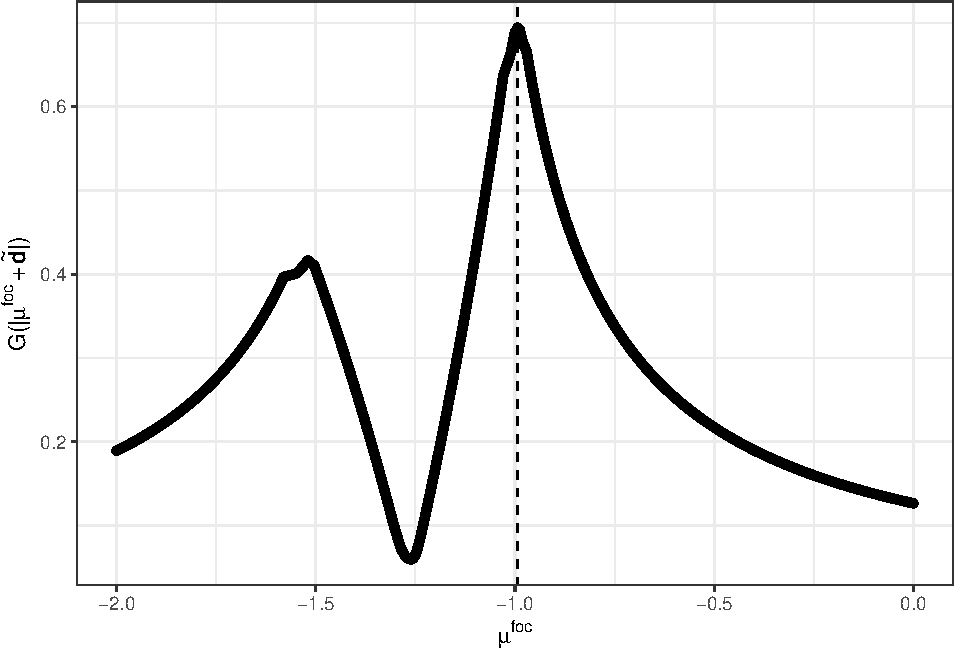
\includegraphics[width=0.7\linewidth]{paper_files/figure-latex/ginipath-1} 

}

\caption{Selecting the anchor point by maximizing the Gini index.}\label{fig:ginipath}
\end{figure}

We then refit the model with the identifying assumption of \(\mu^{\star\text{foc}} = -0.99\). We test each item for DIF and display the results in a MILG as is shown in Figure \ref{fig:ginimilg}.

\begin{verbatim}
## Picking joint bandwidth of 0.00544
\end{verbatim}

\begin{figure}[H]

{\centering 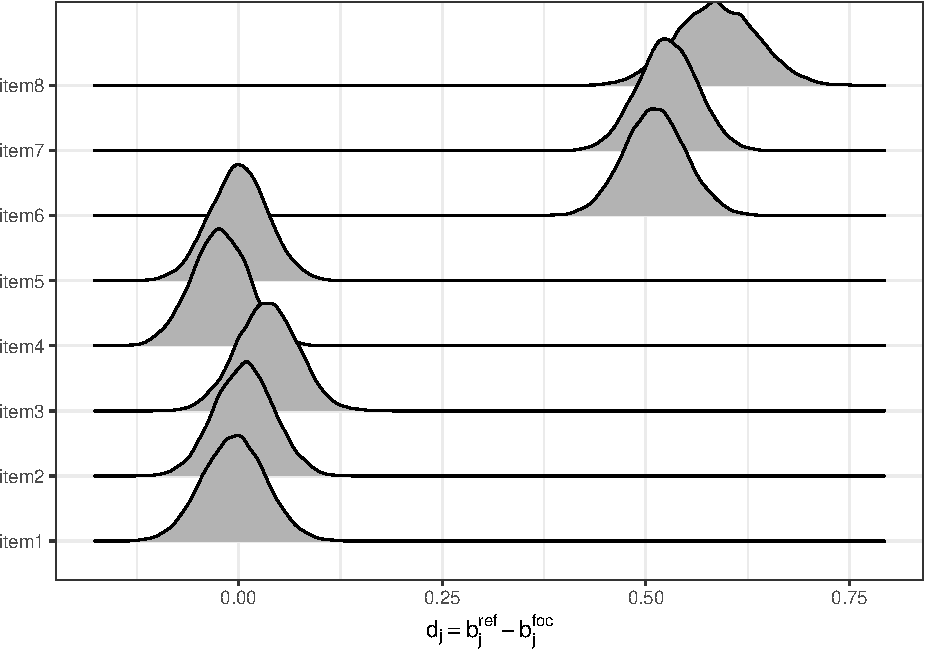
\includegraphics[width=0.7\linewidth]{paper_files/figure-latex/ginimilg-1} 

}

\caption{Selecting the anchor point by maximizing the Gini index.}\label{fig:ginimilg}
\end{figure}

\hypertarget{minimizing-between-curves}{%
\subsubsection{Minimizing between curves}\label{minimizing-between-curves}}

Raju's area method (Raju \protect\hyperlink{ref-raju1988area}{1988}) measures the amount of DIF by calculating the area between the item characteristic curve, the function that maps ability to probability correct response, for each group:
\[
\text{Area Between Curves} = \int |\text{Pr}(y_j = 1| \theta, b_j^{\text{ref}}) - \text{Pr}(y_j = 1| \theta, b_j^{\text{foc}})|
\]
Raju's area method, along with AOAA, have been cited as the two most commonly used IRT-based DIF detection methods (Magis et al. \protect\hyperlink{ref-magis2011generalized}{2011}). We see two weakness of Raju's area method: First, the item characteric curves still need to be linked by anchor items, which the method does not help to identify. Second, the area is unweighted so all values of \(\theta\) matter equally, despite some being much more realistic than others.

Inspired by Raju's area method, we propose a new method, which we call \enquote{minimizing the area between curves} (MABC). To understand MABC, imagine multigroup item response data where \(\mu^{\text{foc}} = \mu^{\text{ref}}\) and \(d_j = 0 \forall j\) so that there is no DIF. The fundamental identification problem of DIF in multigroup IRT models is that there are an infinite number of models with the same likelihood from which to choose. For example, we could correctly assume that the focal group has the same ability as the reference group and fix \(\mu^{\star\text{foc}} = 0\). The model would then estimate \(\hat d_j \approx 0 \forall j\), and we would correctly conclude the groups have the same ability and there is no DIF. Alternatively, we could assume that the focal group has \(\mu^{\star\text{foc}} = 3\). The model would then compensate by finding \(\hat d_j \approx -3 \forall j\), and we would incorrectly conclude that the focal group is high ability but every item contains DIF against them. Both of these models have the same likelihood, so how should one choose which model to believe? MABC chooses the model with the least amount of total DIF, as measured by the total area between the item characteric curves. This is another, perhaps clearer, way of assuming that the majority of items do not contain DIF.

Denote a function that estimates \(\hat b_j^\text{foc}\) by fitting a unidimensional Rasch model where the value of \(\mu^\text{foc}\) is fixed as \(m_j(\mu^\text{foc})\). The amount of DIF on each item is calculated as
\[
\text{DIF}_j(\mu^\text{foc}) = \int |\text{Pr}(y_j = 1| \theta, b_j^{\text{ref}}) - \text{Pr}(y_j = 1| \theta, m_j(\mu^\text{foc}))| g(\theta)d\theta
\]
where \(g(\theta)\) is a weighting function such that \(\int g(\theta)d\theta = 1\). The total DIF on the test, then, is
\[
\text{Total DIF}(\mu^\text{foc}) = \sum_{j} \text{DIF}_j(\mu^\text{foc})
\]
In this way, \(\text{Total DIF}(\mu^\text{foc})\) is a function where the input is \(\mu^\text{foc}\) and the output is the total amount of DIF on the test. MABC sets
\[
\mu^{\star\text{foc}} = \mathop\mathrm{arg\,min}_{\mu^\text{foc}} \text{Total DIF}(\mu^\text{foc}).
\]
MABC is inspired in part by Chalmers, Counsell, and Flora (\protect\hyperlink{ref-chalmers2016might}{2016}) who uses the difference between test characteristic curves weighted by \(g(\theta)\) as a measure of differential test functioning (DTF). The selection of \(g(\theta)\) is important and determines where on the ability spectrum to consider DIF. (\protect\hyperlink{ref-chalmers2016might}{2016}) does not discuss how to choose \(g(\theta)\) and in practice uses \(g(\theta)\) uniform for \(-6 \le \theta \le 6\), which seems like an odd choice. It might seem intuitive to choose \(g(\theta) \sim N(0, 1)\) because \(\mu^\text{ref} = 0\), but this choice doesn't take into account the ability distribution of the focal group. If \(\mu^\text{foc} = 3\), wouldn't we also want to prioritize high \(\theta\) values? We set \(g(\theta)\) to be the average of the reference and focal group ability distributions:
\[
g(\theta) = \dfrac{N(\mu^{\text{ref}}, \sigma^{\text{ref}^2}) + N(\mu^{\text{foc}}, \sigma^{\text{foc}^2})}{2}.
\]

For the simulated data, Figure \ref{fig:mabc} shows Total DIF at a variety of possible values for \(\mu^\text{foc}\). The anchor point is \(\mu^\text{foc} = -1\).

\begin{figure}[H]

{\centering 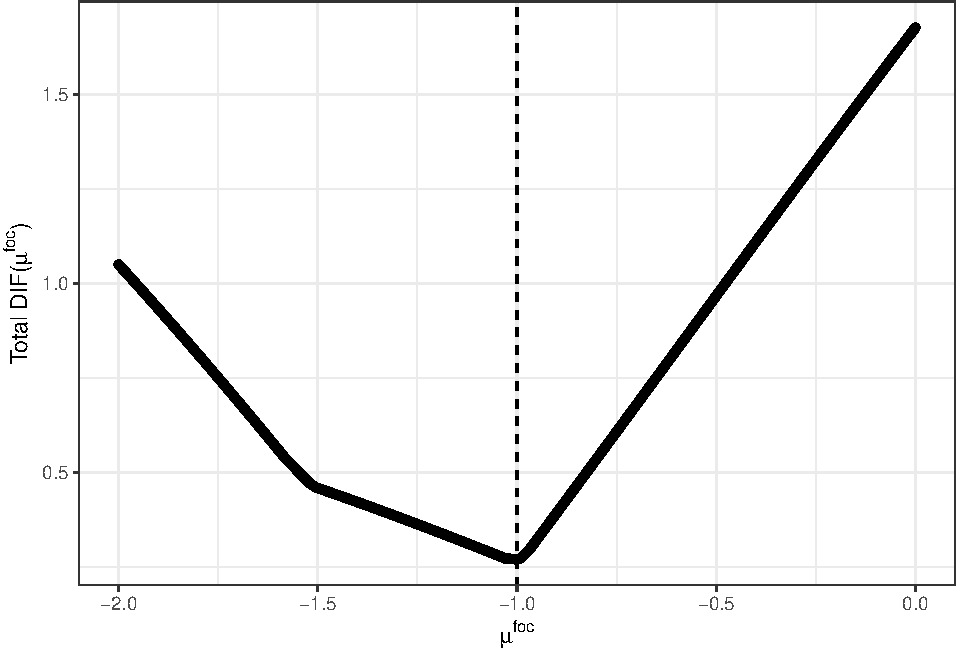
\includegraphics[width=0.7\linewidth]{paper_files/figure-latex/mabc-1} 

}

\caption{Selecting the anchor point by minimizing the total amount of DIF.}\label{fig:mabc}
\end{figure}

\hypertarget{summary}{%
\subsection{Summary}\label{summary}}

{[}ADD A TABLE OF METHODS? OR THAT CAN SORT OF BE DONE IN THE SIMULATION RESULTS?{]}

\hypertarget{next-steps}{%
\section{Next steps}\label{next-steps}}

\hypertarget{remember-my-bounds-idea-i-like-that}{%
\section{Remember my bounds idea I like that}\label{remember-my-bounds-idea-i-like-that}}

\hypertarget{simulate-and-then-walk-through-as-the-analyst-would-with-each-method}{%
\section{Simulate and then walk through as the analyst would with each method}\label{simulate-and-then-walk-through-as-the-analyst-would-with-each-method}}

\hypertarget{mike-frank-example}{%
\section{Mike Frank example}\label{mike-frank-example}}

We know that this test contains DIF. Which items depends on ability difference which we can be sure of. We can, however, quantify the amount of DIF on this test. We can take the SD or we can assume between and calculate chalmers statistic for each. We might not know for sure the ability difference but we can quantify the potential for DIF. For each we calculate the SD across item parameters.

Something with DTF?

Do a simulation where the second dimension varies - a more real testing ground

Example with real data perhaps the Mike Frank data

Summer learning loss as applied DIF?

\clearpage

\hypertarget{notes}{%
\section{Notes}\label{notes}}

\begin{itemize}
\tightlist
\item
  adjust to all be easiness including multidimensional talk
\end{itemize}

\hypertarget{references}{%
\section{References}\label{references}}

\bibliographystyle{apa}
\bibliography{paper.bib}

\hypertarget{refs}{}
\leavevmode\hypertarget{ref-ackerman1992didactic}{}%
Ackerman, Terry A. 1992. ``A Didactic Explanation of Item Bias, Item Impact, and Item Validity from a Multidimensional Perspective.'' \emph{Journal of Educational Measurement} 29 (1): 67--91.

\leavevmode\hypertarget{ref-andrich2012real}{}%
Andrich, David, and Curt Hagquist. 2012. ``Real and Artificial Differential Item Functioning.'' \emph{Journal of Educational and Behavioral Statistics} 37 (3): 387--416.

\leavevmode\hypertarget{ref-bechger2015statistical}{}%
Bechger, Timo M, and Gunter Maris. 2015. ``A Statistical Test for Differential Item Pair Functioning.'' \emph{Psychometrika} 80 (2): 317--40.

\leavevmode\hypertarget{ref-camilli1992conceptual}{}%
Camilli, Gregory. 1992. ``A Conceptual Analysis of Differential Item Functioning in Terms of a Multidimensional Item Response Model.'' \emph{Applied Psychological Measurement} 16 (2): 129--47.

\leavevmode\hypertarget{ref-chalmers2018numerical}{}%
Chalmers, R Philip. 2018. ``Numerical Approximation of the Observed Information Matrix with Oakes' Identity.'' \emph{British Journal of Mathematical and Statistical Psychology} 71 (3): 415--36.

\leavevmode\hypertarget{ref-chalmers2016might}{}%
Chalmers, R Philip, Alyssa Counsell, and David B Flora. 2016. ``It Might Not Make a Big Dif: Improved Differential Test Functioning Statistics That Account for Sampling Variability.'' \emph{Educational and Psychological Measurement} 76 (1): 114--40.

\leavevmode\hypertarget{ref-chitiga2015income}{}%
Chitiga, Margaret, E Sekyere, and N Tsoanamatsie. 2015. ``Income Inequality and Limitations of the Gini Index: The Case of South Africa.'' \emph{Human Sciences Research Council (HSRC), Available at: Http://Www. Hsrc. Ac. Za/En/Review/Hsrc-Review-November-2014/Limitations-of-Gini-Index, Site Accessed} 2.

\leavevmode\hypertarget{ref-drasgow1987study}{}%
Drasgow, Fritz. 1987. ``Study of the Measurement Bias of Two Standardized Psychological Tests.'' \emph{Journal of Applied Psychology} 72 (1): 19.

\leavevmode\hypertarget{ref-edelen2006identification}{}%
Edelen, Maria Orlando, David Thissen, Jeanne A Teresi, Marjorie Kleinman, and Katja Ocepek-Welikson. 2006. ``Identification of Differential Item Functioning Using Item Response Theory and the Likelihood-Based Model Comparison Approach: Application to the Mini-Mental State Examination.'' \emph{Medical Care}, S134--S142.

\leavevmode\hypertarget{ref-gini1912variabilita}{}%
Gini, Corrado. 1912. ``Variabilità E Mutabilità (Variability and Mutability).'' \emph{Tipografia Di Paolo Cuppini, Bologna, Italy}, 156.

\leavevmode\hypertarget{ref-hastie2001estimating}{}%
Hastie, Trevor, Robert Tibshirani, and Guenther Walther. 2001. ``Estimating the Number of Data Clusters via the Gap Statistic.'' \emph{J Roy Stat Soc B} 63: 411--23.

\leavevmode\hypertarget{ref-holland1986differential}{}%
Holland, Paul W, and Dorothy T Thayer. 1986. ``Differential Item Functioning and the Mantel-Haenszel Procedure.'' \emph{ETS Research Report Series} 1986 (2): i--24.

\leavevmode\hypertarget{ref-kopf2015framework}{}%
Kopf, Julia, Achim Zeileis, and Carolin Strobl. 2015. ``A Framework for Anchor Methods and an Iterative Forward Approach for Dif Detection.'' \emph{Applied Psychological Measurement} 39 (2): 83--103.

\leavevmode\hypertarget{ref-magis2011generalized}{}%
Magis, David, Gilles Raı̂che, Sébastien Béland, and Paul Gérard. 2011. ``A Generalized Logistic Regression Procedure to Detect Differential Item Functioning Among Multiple Groups.'' \emph{International Journal of Testing} 11 (4): 365--86.

\leavevmode\hypertarget{ref-meade2012solving}{}%
Meade, Adam W, and Natalie A Wright. 2012. ``Solving the Measurement Invariance Anchor Item Problem in Item Response Theory.'' \emph{Journal of Applied Psychology} 97 (5): 1016.

\leavevmode\hypertarget{ref-pohl2017cluster}{}%
Pohl, Steffi, Eric Stets, and Claus H Carstensen. 2017. ``CluStEr-baSEd anCHor Item Identification and Selection.'' NEPS Working Paper.

\leavevmode\hypertarget{ref-raju1988area}{}%
Raju, Nambury S. 1988. ``The Area Between Two Item Characteristic Curves.'' \emph{Psychometrika} 53 (4): 495--502.

\leavevmode\hypertarget{ref-stark2006detecting}{}%
Stark, Stephen, Oleksandr S Chernyshenko, and Fritz Drasgow. 2006. ``Detecting Differential Item Functioning with Confirmatory Factor Analysis and Item Response Theory: Toward a Unified Strategy.'' \emph{Journal of Applied Psychology} 91 (6): 1292.

\leavevmode\hypertarget{ref-strobl2018anchor}{}%
Strobl, Carolin, Julia Kopf, Raphael Hartmann, and Achim Zeileis. 2018. ``Anchor Point Selection: An Approach for Anchoring Without Anchor Items.'' Working Papers in Economics; Statistics.

\leavevmode\hypertarget{ref-swaminathan1990detecting}{}%
Swaminathan, Hariharan, and H Jane Rogers. 1990. ``Detecting Differential Item Functioning Using Logistic Regression Procedures.'' \emph{Journal of Educational Measurement} 27 (4): 361--70.

\leavevmode\hypertarget{ref-talbot2013taking}{}%
Talbot III, Robert M. 2013. ``Taking an Item-Level Approach to Measuring Change with the Force and Motion Conceptual Evaluation: An Application of Item Response Theory.'' \emph{School Science and Mathematics} 113 (7): 356--65.

\leavevmode\hypertarget{ref-thissen1993detection}{}%
Thissen, David, Lynne Steinberg, and Howard Wainer. 1993. ``Detection of Differential Item Functioning Using the Parameters of Item Response Models.''

\leavevmode\hypertarget{ref-woods2009empirical}{}%
Woods, Carol M. 2009. ``Empirical Selection of Anchors for Tests of Differential Item Functioning.'' \emph{Applied Psychological Measurement} 33 (1): 42--57.

\leavevmode\hypertarget{ref-yang2012characterizing}{}%
Yang, Ji Seung, Mark Hansen, and Li Cai. 2012. ``Characterizing Sources of Uncertainty in Item Response Theory Scale Scores.'' \emph{Educational and Psychological Measurement} 72 (2): 264--90.

\end{document}
